%
% Chapter 3 - Results
%
\chapter{Results}
This chapter shows the final results of this project.\\

All options and decisions made by the group will be displayed in the sections below, as every relevant detail of each developed module.

\newpage
\section{Relational database}

\subsection{Used tecnologies}

When the project was in a planning phase, the group decided that a relational database was the most suitable option for this project
instead of a No-SQL database, because of the project's structure - there are many hierarchies between entities, which invalidated the
no-SQL option.\\

After some discussion about the tecnology to be used, the group chose to use PostgreSQL rather than Microsoft SQL, because it has the
PostGIS plugin which is convenient for geolocation proposes and it is supported by an Heroku plugin, where it is planned to deploy the
front end web application alongside with the database model.\\

\subsection{Conceptual model}
As a result of multiples redesigns, here is the database's conceptual model.

\begin{figure}[H]    
    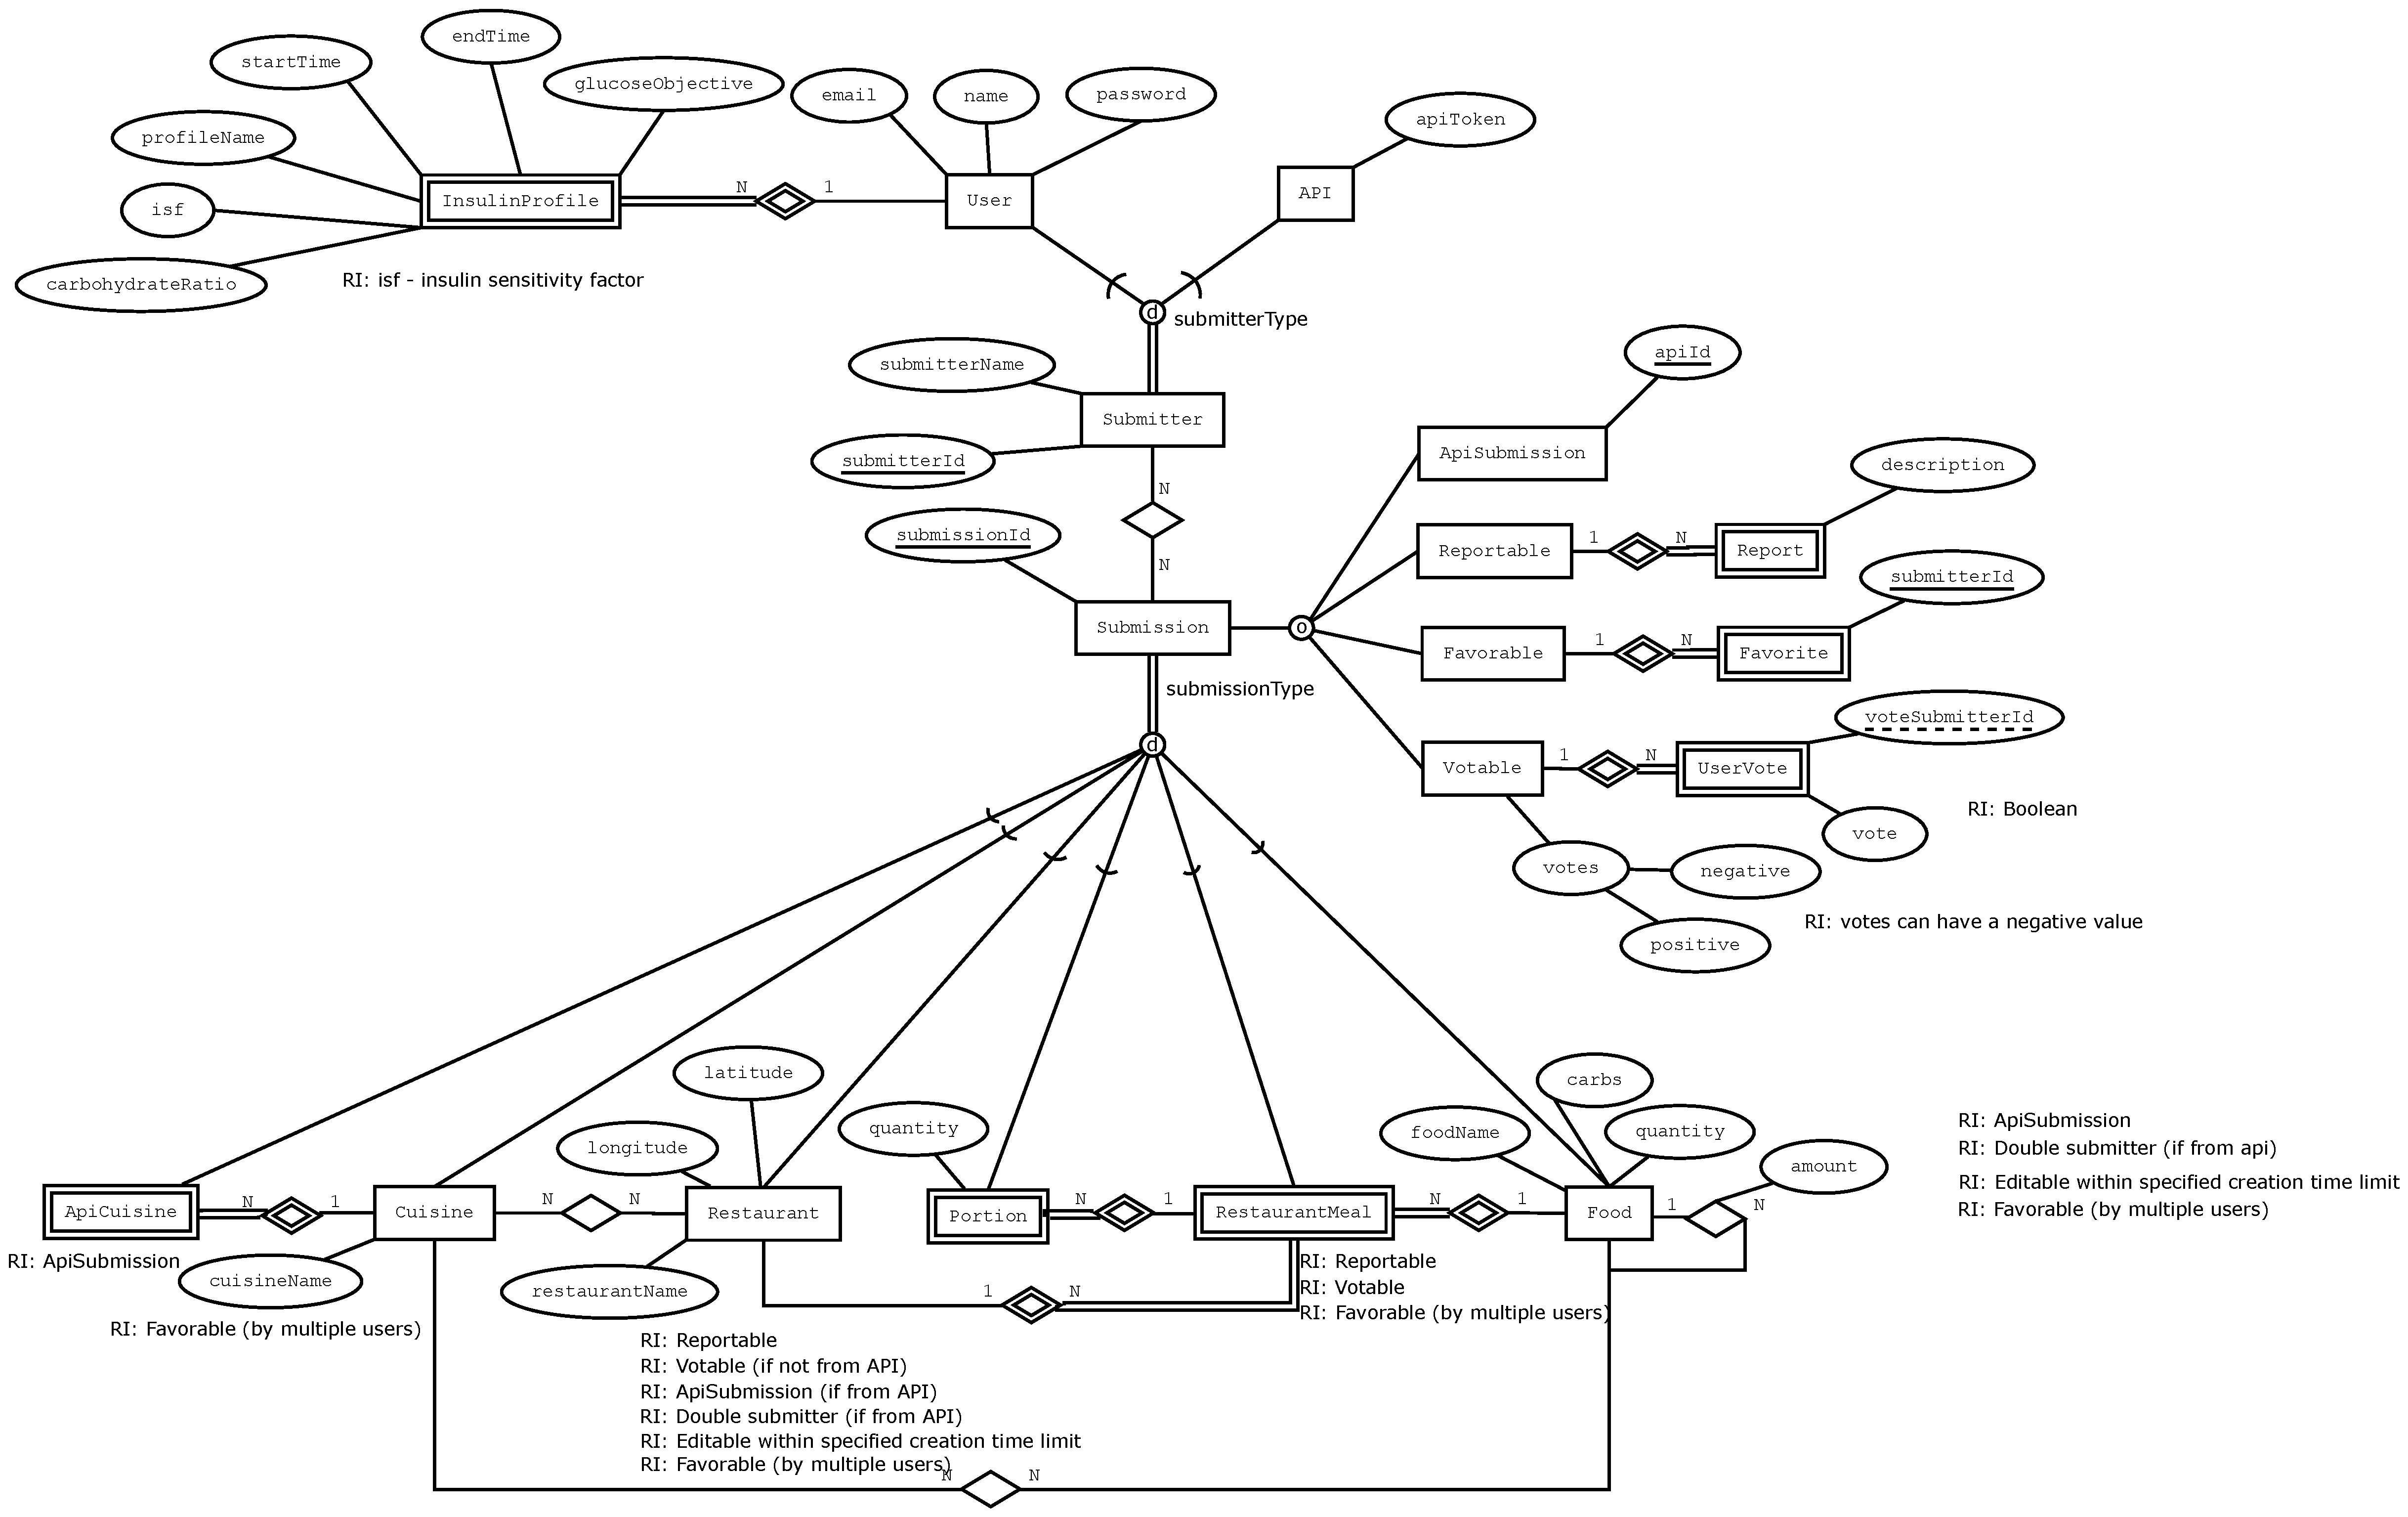
\includegraphics[scale=0.2]{_figures/Nutr.io_Database_Diagram.eps}
    \caption{Database conceptual model}
\end{figure}

The database's relational model is present inside this report's appendix [\nameref{app:relational_model}].\\

In the relational model there are tables which are not specified in the conceptual model.
These are a product from associations between entities which will simplify queries' complexity.\\

Now the submission can fall into 4 categories: ApiSubmission, Reportable, Favorable and Votable, in order to disguish between submissions that
are from the user or from APIs and to separate which ones can be reportable, favorable and votable by the user.\\

The cuisine entity has now an associated entity called ApiCuisine, to save cuisine information provided by the Here API.\\

Meals and ingredients were now condensed into one entity called food - now each meal can have meals inside it that can also be considered
ingredients in other contexts.\\

Therefore each meal possesses nutritional information, which is essential to the user especially to the insulin calculations. That information is composed by
'carbs' - meal's carbohydrates; and quantity - meal's quantity.\\

\section{HTTP server}

\subsection{Used tecnologies}

\subsubsection{Kotlin}

The group chose to use Kotlin for the HTTP server developed as it is a language that is being more adopted and used nowadays and because it is totally 
interoperable with Java.\\

It was also the language used during PDM, which is an optional course for Android application development inside the LEIC programme, 
making this a language the group felt confortable with.\\

\subsubsection{Spring MVC}

At the beginning of the project the group decided to use Spring MVC rather than Ktor, as the first one is taught in DAW, which is an optional course
for Web applications development inside the LEIC programme. As Spring MVC has a better coverage inside the LEIC programme, the group considered 
it a more solid choice.\\

\subsubsection{Used dependencies}

\textbf{TODO - eng. Félix says: "external dependencies used."}\\

Here are all the dependencies injected inside HTTP server gradle settings file.\\

\begin{itemize}
    \item \textbf{Kotlin base dependencies} - kotlin-reflect and kotlin-stdlib-jdk8;
    \item \textbf{Spring base dependencies} - spring-boot-starter and starter-web;
    \item \textbf{Mockito} - for tests with mocks;
    \item \textbf{Jackson} - for JSON serialization and deserialization;
    \item \textbf{JDBI} - the driver/interface for connecting with the relational database;
    \item \textbf{Spring Security} - for authentication and authorization proposes.
\end{itemize}

\subsection{Code structure}

\textbf{TODO - eng. Félix says: "Needs more information about the backend organization, such as: intermediaries, controllers, services, database access method, external dependencies used"}

\subsection{JDBI}

After some discussion of which driver should be used to allow communication between the server and database, the group decided that the JDBI was best
option as it is a library built on JDBC.\\

The library also exposes two different API's styles: a fluent style and sql object style (used during development), as shown below.

\begin{figure}[H]
    \begin{center}
        \includegraphics[scale=0.5]{_figures/fluentApiJdbi.png}
        \caption{JDBI using a fluent API style}
    \end{center}
\end{figure}

\begin{figure}[H]
    \begin{center}
        \includegraphics[scale=0.5]{_figures/sqlObjectJdbi.png}
        \caption{JDBI using a SQL object API style (example from HTTP server)}
    \end{center}
\end{figure}

\textbf{TODO - eng. Félix says: "Usage of JDBI and the declarative API needs justification and perhaps a brief introduction."}

\section{Geolocation}

Given how all clients rely on obtaining nearby restaurants, there was a need to implement a geolocation function in the project's design.\\

Initial research showcased two possible solutions: Haversine distances and cartesian distances, where the latter returns a highly imprecise distances.
As such, Haversine was selected.\\

The next step was to choose which system filters nearby restaurants: database or HTTP server. After some discussion, the group decided that database was the best
option for two reasons: 
\begin{itemize}
    \item Given the large amount of existing restaurants, sending such data from the database to the HTTP server so that it could filter it would occupy too much memory;
    \item PostgreSQL already supplies extensions that add support for location queries, namely PostGIS.
\end{itemize}

\section{Android application}

\subsection{Used tecnologies}

\subsubsection{Kotlin}

The group chose to use Kotlin for the mobile application development, as it is now the official programming language for Android development,
according to Google.\\

\subsubsection{External dependencies}

Here are the dependencies that were included in the mobile application which gave more functionalities to it.

\begin{itemize}
    \item \textbf{Volley} - an HTTP library for Android networking;
    \item \textbf{Jackson} - JSON serialization, deserialization and handling;
    \item \textbf{Room} - A framework to store data locally;
    \item \textbf{MapBox} - A framework to provide maps and geolocation tools;
    \item \textbf{MPAndroidChart} - provides custom graphs inside the application;
    \item \textbf{Glide} - a framework for image loading.
\end{itemize}

\subsection{Code structure}

\subsubsection{Drawing pattern}

The mobile application code structure follows the \textbf{repository pattern}, which is a code architecture recommended by the \textbf{Android Jetpack} for this type of applications.\\

\begin{figure}[H]
    \begin{center}
        \includegraphics[scale=0.5]{_figures/repository_pattern2.png}
        \caption{The repository pattern diagram}
    \end{center}
\end{figure}

Above there is the pattern's diagram provided by the Android Jetpack.\\

The idea behind this architecture is that each Activity or fragment has its own ViewModel and each one calls the needed functions present inside the repository.
The repository corresponds to a layer that manages where the information should be retrieved from.\\

The 'DTO to model' mapping also occurs inside the repository, following the rule where ViewModels should only manipulate models and the layers below should only use DTOs.\\

The application follows this diagram with the only difference that Volley is used instead of Retrofit.\\

By following this pattern, the code becomes segmented and organized,
allowing a good comprehension and code maintainability.\\

\subsubsection{Local data storing}

As mentioned in the dependencies, the mobile application utilizes Room to store data locally. This is convenient
for multiple reasons: 
\begin{itemize}
    \item To allow using the application in offline situations;
    \item To save data in order to avoid unnecessary requests to the server;
    \item To help data synchronization, that will be detailed later in this section.
\end{itemize}

\subsubsection{User authentication and authorization}

The user has the ability to sign up or sign in the mobile application. Besides being the server responsable for this matter, the mobile application has also some intervention
here, because after a successful login or register, the HTTP server will return a jwt (JSON Web Token) that will authenticate and authorize the user in future requests.\\

This token will be stored in the Android SharedPreferences, which is the safest way to store a token inside Android applications. The token will also to be renewed from time
to time due to expiration time.

\subsubsection{Data synchronization}

Background data synchronization will happen after a successful login or register. The only user data that will be synchronized are:
\begin{itemize}
    \item Insulin profiles;
    \item Custom meals made by the user;
    \item Favorites.
\end{itemize}

When logged in, the data can be synchronized in two ways: the user forces the synchronization by triggering a button inside the specific list;
The Android WorkManager will make sure that the data is synchronized at least once a 
day when the phone is inactive and connected to the internet.

\subsubsection{Android version compatibility}

In order to garantee a global support by most of the Android devices nowadays, the mobile application is supported since \textbf{Android 7} (API level 24)
up to \textbf{Android 10} (API level 29). It is recommended to use the last one as the Android emulator used this version.

\subsubsection{TODO}
As mentioned in the progress report, the group managed to implement in the mobile application a fragment that displays a map with a list of restaurants nearby the user.\\

The user can also search for restaurants, meals and cuisines providing the associated name or identifier.\\

The core feature of the application was also finished during this time period - the insulin calculator. This feature calculates how many insulin doses should be injected
in order to maintain the blood glucose levels stabilized according to the user's planned glucose objective for that period of the day.\\

The blood glucose objective is set inside the user's profile, by creating multiples insulin profiles, each one has a limited time period to give the user freedom to map its
own insulin routine throughout the day.\\

This is due to the fact that user's insulin sensitivity factor varies along the day, so the user has the ability to specify its own values in order to the calculator\\
